% =====================================================================================================
% NARRATIVE OUTLINE: the flow of the paper, told as a story.
%
% Each paragraph below is one beat of the story: what the reader must learn at that point, and why the
% next paragraph follows. The prose is a first form of the final text, not the final text. Language is
% simple technical English (short sentences, active voice, one idea in each sentence).
%
% Model for the narrative: Bourtsoulatze, Kurka & Gunduz, "Deep Joint Source-Channel Coding for Wireless
% Image Transmission" (2019). That paper opens with the separation theorem, shows its practical limit
% (the cliff), offers one clear idea, and then lets each experiment answer the next obvious question.
% We use the same arc. Section layout follows ADJSCC (system model, method with one architecture
% figure, experiments, conclusion).
%
% Other versions in this folder: main_detailed_draft.tex (all results, full tables),
% main_outline_bullets.tex (bullet outline). Numbers and their sources: RESULTS_COMPENDIUM.md.
% =====================================================================================================
\documentclass[journal]{IEEEtran}
\usepackage{amsmath,amssymb,amsthm}
\usepackage{graphicx}
\usepackage{booktabs}
\usepackage{xcolor}
\usepackage{cite}
\usepackage{url}
\usepackage{pifont}
\usepackage{tikz}
\usetikzlibrary{positioning,arrows.meta,calc}

\newtheorem{lemma}{Lemma}
\newtheorem{proposition}{Proposition}
\providecommand{\TBD}[1]{\textbf{\color{red}[#1]}}
\newcommand{\beat}[1]{\noindent\textcolor{blue!60!black}{\textsf{\footnotesize [#1]}}\ }

\graphicspath{{../results/}{../published_results/}{../paper/figures/}{figures/}}
\newcommand{\figbox}[2]{%
  \fbox{\parbox[c][3.2cm][c]{\dimexpr#1-2\fboxsep-2\fboxrule\relax}{\centering\footnotesize\color{gray}\textbf{FIGURE TO MAKE}\\[2pt]#2}}}
\newcommand{\resfig}[3]{%
  \IfFileExists{../results/#2}{\includegraphics[width=#1]{#2}}{%
  \IfFileExists{../published_results/#2}{\includegraphics[width=#1]{#2}}{%
  \IfFileExists{../paper/figures/#2}{\includegraphics[width=#1]{#2}}{\figbox{#1}{#3\\(\texttt{#2})}}}}}

\begin{document}

\title{Which Latent Bytes Need Parity? Importance-Aware Reed--Solomon Protection of Deep JSCC Latents
for Images, Speech and Text}
\author{\TBD{Authors}}
\maketitle

% -----------------------------------------------------------------------------------------------------
% THE STORY IN SEVEN SENTENCES (read this first; every section serves one of these sentences)
%  1. Deep JSCC removed the cliff of separate coding, but packet networks bring it back.
%  2. To cross a packet network, a latent becomes bytes, and the bytes need Reed-Solomon parity.
%  3. With a fixed parity budget, a classical question returns: which bytes deserve the parity?
%  4. The classical answer needs a known order of importance; a JSCC latent hides its order.
%  5. We measure the order: it is real and strong for images and speech, and attention does not see it.
%  6. Once the order is known, the best use of the parity is simple: send the important channels with
%     one strong code, and do not send the rest.
%  7. The same measurement also tells when not to bother: for text, the order is flat.
% -----------------------------------------------------------------------------------------------------

\begin{abstract}
\beat{1. Context}
Deep joint source-channel coding (JSCC) gives a graceful loss of quality when the channel becomes worse.
\beat{2. Tension}
Packet networks lose full packets, so a deep JSCC latent must travel as bytes with packet-level
Reed--Solomon (RS) parity, and the cliff of the code returns.
\beat{3. Question}
With a fixed parity budget, which latent bytes must get the parity?
\beat{4. Method}
We quantize the latents of image, speech and text models to the same $16\times64$-byte format and measure
how much each latent channel damages the output when it is lost.
\beat{5. Findings}
For images and speech, four of 16 channels cause 33--53\% of the damage. The attention gates of the
network do not find these channels; latent energy and a static table do. With this order, the best use
of the parity is truncation: at 40\% packet loss it gives 6.5~dB more than equal protection for images.
For text, the damage is almost equal, and equal protection stays the correct choice.
\beat{6. Message}
Measure what ``important'' means before you protect it.
\end{abstract}

% =====================================================================================================
\section{Introduction}
% Arc of the introduction (as in the Deep JSCC paper): a known principle -> its practical limit ->
% the new setting where the limit returns -> the question -> why the obvious answer is not enough ->
% what we do -> what we find -> contributions.

\beat{P1. The promise of deep JSCC}
Shannon's separation theorem says that source coding and channel coding can be designed apart without
loss, but only for very long blocks. Practical systems pay for this: when the channel becomes worse than
the code can correct, the decoder fails at once. This is the ``cliff effect''. Deep JSCC removes the cliff:
one neural network maps the source to channel symbols, and its quality decreases slowly as the channel
becomes worse \cite{bourtsoulatze2019deep}. Later work adds SNR-adaptive attention \cite{xu2022adjscc}
and quantized, digital latents \cite{tung2022deepjsccq}.

\beat{P2. The setting where the cliff returns}
Most deep JSCC studies assume a noisy physical channel. Many real links are different. An application
gives bytes to the network, the network sends them in packets, and congestion or interference removes
full packets. The receiver knows which packets are missing. To use such a link, the latent must become
bytes, and the bytes need packet-level forward error correction. Reed--Solomon (RS) codes are the natural
choice: an RS$(n,k)$ code recovers its data from any $k$ of its $n$ symbols. But an RS code has a cliff
too. The graceful loss of quality that made deep JSCC attractive is lost again at the packet layer.

\beat{P3. The question}
If the parity budget is fixed, it can protect some bytes more than others. This raises an old question
in a new form: which latent bytes deserve the parity? For layered image and video codecs, unequal loss
protection answered this question long ago \cite{albanese1996pet,mohr2000ulp,dumitrescu2004optimal}.
Those answers depend on one property: the bit stream has a known order of importance.

\beat{P4. Why the old answer does not transfer, and the obvious shortcut}
A JSCC latent has no known order. The training does not ask the network to put important information
in a particular channel. Recent work takes importance from attention weights or saliency maps
\cite{uyanik2023gradfec,zhan2026isfr}. This is attractive because ADJSCC already computes one attention
weight for each channel. But nobody has checked if these weights tell which channel causes the most
damage when it is lost.

\beat{P5. What we do}
We study the question with one common latent format for three sources: images, speech and text. Each
model maps a sample to 16 channels of 64 one-byte values, and the same RS packetizer sends them in 96
packets. We train each model with and without attention modules. We erase one channel at a time and
measure the damage, and we use this measurement to decide where the parity goes.

\beat{P6. What we find (the answers, in the order the paper shows them)}
First, the damage is very unequal for images and speech, but almost equal for text. Second, attention
does not find the important channels; simple statistics of the latent do. Third, once the order is
known, the best allocation is not many protection levels: it is to send the important channels with one
strong code and to drop the rest. Fourth, the order gives almost all of the gain. A random order gives
very little.

\beat{P7. Contributions}
\begin{enumerate}
\item A byte-level JSCC pipeline with importance-aware RS protection that works the same way for
images, speech and text (Fig.~\ref{fig:workflow}).
\item A measurement of erasure sensitivity in three modalities, with and without attention.
\item Evidence that attention gates do not predict erasure damage, and cheap predictors that do.
\item An exact model of RS outcomes and an optimal parity allocation.
\item Criteria, fixed before the test, that tell when unequal protection is useful, and one modality
(text) where it is not.
\end{enumerate}

\beat{P8. Road map}
Section~\ref{sec:related} places the work. Section~\ref{sec:model} defines the system and the question.
Section~\ref{sec:method} describes the pipeline. Section~\ref{sec:exp} answers the questions in order,
first for images, then for speech and text. Section~\ref{sec:conclusion} concludes.

% =====================================================================================================
\section{Related Work}\label{sec:related}
% Role in the story: show the three threads that meet in this paper, and the gap where they meet.
% Keep it short. Each paragraph ends with what that thread does NOT answer.

\beat{R1. Deep JSCC: from analog to digital}
Deep JSCC began with images over noisy channels \cite{bourtsoulatze2019deep} and grew to bandwidth-agile
\cite{kurka2021bandwidth}, SNR-adaptive \cite{xu2022adjscc} and quantized \cite{tung2022deepjsccq} forms.
Recent work trains latents to survive lost packets without parity \cite{esfahanizadeh2026block,
bo2026lgsemcom,wei2026everypacket}. Semantic systems also send text and speech \cite{xie2021deepsc,
weng2021deepscs}. These studies do not ask how to share a parity budget across the latent.

\beat{R2. Unequal protection: the classical answer}
PET \cite{albanese1996pet} and optimal unequal loss protection \cite{mohr2000ulp,dumitrescu2004optimal,
hamzaoui2005optimized} share parity across a progressive bit stream. They assume the order is known.

\beat{R3. Importance of learned features}
Grad-FEC \cite{uyanik2023gradfec} and ISFR \cite{zhan2026isfr} rank learned features for protection.
Studies in machine learning show that attention weights often do not predict what happens when a
feature is removed \cite{jain2019attention,morcos2018single}. Our work joins these threads: it measures
the order, tests attention as a shortcut, and finds the best way to use the order.

% =====================================================================================================
\section{System Model}\label{sec:model}
% Role in the story: make the question precise. One figure, a few symbols, one problem statement.
% The reader should leave this section knowing exactly what is fixed (network, 96 packets) and what
% we may choose (channel order, code layout).

\begin{figure}[t]\centering
\resizebox{\columnwidth}{!}{%
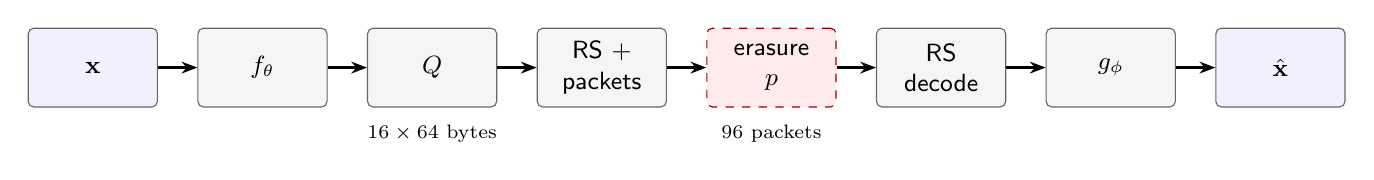
\begin{tikzpicture}[font=\sffamily\small, >={Stealth[length=2mm]}, node distance=4mm and 5mm,
  b/.style={draw=black!60, fill=black!4, rounded corners=2pt, align=center, minimum height=10mm, text width=15mm, inner sep=2pt},
  c/.style={b, fill=red!8, draw=red!60!black, dashed}]
\node[b, fill=blue!6] (x) {$\mathbf{x}$};
\node[b, right=of x] (f) {$f_\theta$};
\node[b, right=of f] (q) {$Q$};
\node[b, right=of q] (e) {RS +\\packets};
\node[c, right=of e] (ch) {erasure\\$p$};
\node[b, right=of ch] (d) {RS\\decode};
\node[b, right=of d] (g) {$g_\phi$};
\node[b, fill=blue!6, right=of g] (xh) {$\hat{\mathbf{x}}$};
\foreach \a/\b in {x/f,f/q,q/e,e/ch,ch/d,d/g,g/xh} \draw[->, thick] (\a) -- (\b);
\node[below=1mm of q, font=\scriptsize] {$16\times64$ bytes};
\node[below=1mm of ch, font=\scriptsize] {96 packets};
\end{tikzpicture}}
\caption{System model.}\label{fig:system}
\end{figure}

\beat{S1. From source to bytes}
An encoder $f_\theta$ maps a source sample $\mathbf{x}$ to 16 latent channels of 64 values. A learned
quantizer $Q$ maps each value to one byte, which is also one RS symbol (Fig.~\ref{fig:system}). The
source is an image, a speech segment or a text window (Table~\ref{tab:modalities}); the latent format
is the same for all three.

\begin{table}[t]\centering\caption{Three sources, one latent format}\label{tab:modalities}
\resizebox{\columnwidth}{!}{%
\begin{tabular}{llll}\toprule
 & Image & Speech & Text\\\midrule
Dataset & CIFAR-10 & LibriSpeech & text8\\
Sample & $32\times32$ image & 1.024~s segment & 2,048 characters\\
Latent & \multicolumn{3}{c}{16 channels $\times$ 64 bytes $=1{,}024$ bytes}\\
Quality & PSNR (dB) & SNR (dB) & character accuracy (\%)\\
\bottomrule\end{tabular}}
\end{table}

\beat{S2. From bytes to packets}
The transmitter has 96 packets of 16 bytes: 64 packets of data and 32 packets of parity. Each packet
carries one symbol of each codeword, so a lost packet costs each codeword one symbol. The channel loses
each packet with probability $p$, and the receiver knows which packets are missing.

\beat{S3. The question in one line}
The network is fixed and the number of packets is fixed. We may choose two things: the order of the
channels and the RS code for each group of channels. We want the choice that gives the best expected
quality. With equal protection, one RS(96,64) code covers all channels and survives up to 33\% loss.
The rest of the paper asks if a better choice exists.

% =====================================================================================================
\section{Importance-Aware RS Protection}\label{sec:method}
% Role in the story: give the reader the tools, in the order the experiments will use them:
% (1) a way to measure importance, (2) ways to predict it, (3) a way to compute the effect of any
% code layout exactly, (4) a way to choose the layout. Open with the one architecture figure.

\begin{figure*}[t]\centering
\resizebox{\textwidth}{!}{%
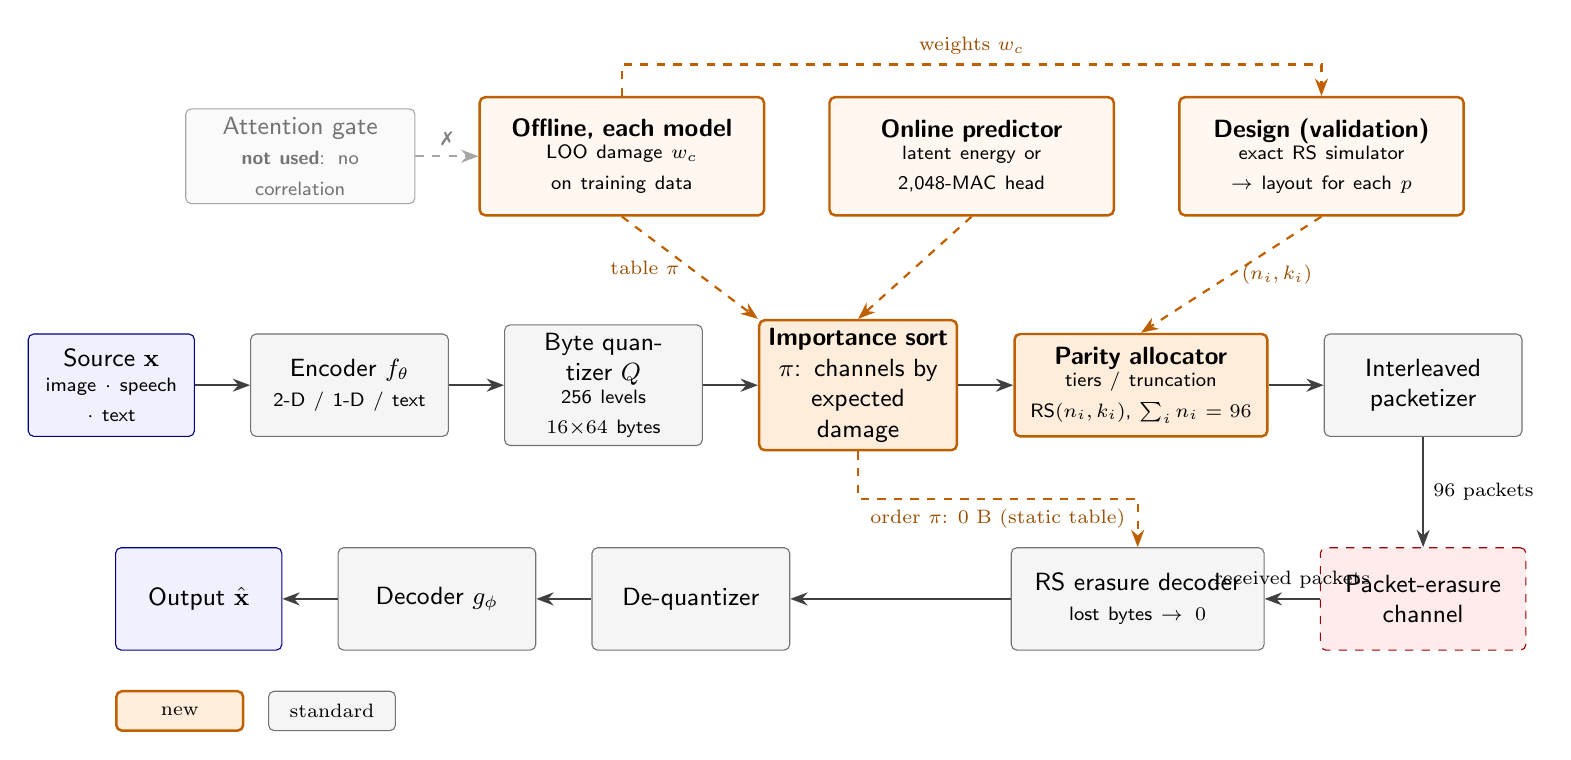
\begin{tikzpicture}[
  font=\sffamily\small, >={Stealth[length=2.2mm]}, node distance=6mm and 7mm,
  std/.style={draw=black!55, fill=black!4, rounded corners=2pt, align=center, minimum height=13mm,
              text width=23mm, inner sep=3pt},
  new/.style={std, draw=orange!75!black, fill=orange!14, line width=0.9pt},
  src/.style={std, text width=19mm, fill=blue!6, draw=blue!50!black},
  chan/.style={std, fill=red!8, draw=red!60!black, dashed, text width=24mm},
  off/.style={new, fill=orange!6, text width=34mm, minimum height=15mm},
  bad/.style={std, fill=black!2, draw=black!35, text=black!55, text width=27mm, minimum height=10mm},
  flow/.style={->, line width=0.8pt, draw=black!75},
  side/.style={->, line width=0.8pt, draw=orange!75!black, dashed}]
\node[src] (x) {Source $\mathbf{x}$\\[1pt]\scriptsize image $\cdot$ speech\\\scriptsize $\cdot$ text};
\node[std, right=of x] (enc) {Encoder $f_\theta$\\\scriptsize 2-D / 1-D / text};
\node[std, right=of enc] (q) {Byte quantizer $Q$\\\scriptsize 256 levels\\\scriptsize $16{\times}64$ bytes};
\node[new, right=of q] (sort) {\textbf{Importance sort}\\$\pi$: channels by\\expected damage};
\node[new, right=of sort, text width=30mm] (alloc) {\textbf{Parity allocator}\\\scriptsize tiers / truncation\\\scriptsize RS$(n_i,k_i)$, $\sum_i n_i = 96$};
\node[std, right=of alloc] (pkt) {Interleaved\\packetizer};
\node[chan, below=14mm of pkt] (ch) {Packet-erasure\\channel};
\node[std, left=of ch, text width=30mm] (rsdec) {RS erasure decoder\\\scriptsize lost bytes $\to 0$};
\node[std, left=of rsdec, xshift=-21mm] (deq) {De-quantizer};
\node[std, left=of deq] (dec) {Decoder $g_\phi$};
\node[src, left=of dec] (xh) {Output $\hat{\mathbf{x}}$};
\node[off, above=13mm of sort, xshift=-30mm] (loo) {\textbf{Offline, each model}\\\scriptsize LOO damage $w_c$\\\scriptsize on training data};
\node[off, right=8mm of loo] (proxy) {\textbf{Online predictor}\\\scriptsize latent energy or\\\scriptsize 2,048-MAC head};
\node[off, right=8mm of proxy] (sim) {\textbf{Design (validation)}\\\scriptsize exact RS simulator\\\scriptsize $\to$ layout for each $p$};
\node[bad, left=8mm of loo] (att) {Attention gate\\\scriptsize \textbf{not used}: no correlation};
\draw[flow] (x) -- (enc); \draw[flow] (enc) -- (q); \draw[flow] (q) -- (sort);
\draw[flow] (sort) -- (alloc); \draw[flow] (alloc) -- (pkt);
\draw[flow] (pkt) -- node[right, font=\scriptsize] {96 packets} (ch);
\draw[flow] (ch) -- node[above, font=\scriptsize] {received packets} (rsdec);
\draw[flow] (rsdec) -- (deq); \draw[flow] (deq) -- (dec); \draw[flow] (dec) -- (xh);
\draw[side] (loo.south) -- node[left, font=\scriptsize, text=orange!60!black] {table $\pi$} (sort.north west);
\draw[side] (proxy.south) -- (sort.north);
\draw[side] (sim.south) -- node[right, font=\scriptsize, text=orange!60!black] {$(n_i,k_i)$} (alloc.north);
\draw[side] (loo.north) |- ++(0,4mm) -| node[pos=0.25, above, font=\scriptsize, text=orange!60!black] {weights $w_c$} (sim.north);
\draw[->, line width=0.8pt, draw=black!35, dashed] (att.east) -- node[above, font=\scriptsize, text=black!50] {\ding{55}} (loo.west);
\draw[side] (sort.south) -- ++(0,-6mm) -| node[pos=0.25, below, font=\scriptsize, text=orange!60!black]
      {order $\pi$: 0 B (static table)} (rsdec.north);
\node[new, text width=14mm, minimum height=5mm, below=5mm of xh.south west, anchor=north west, font=\scriptsize] (l1) {new};
\node[std, text width=14mm, minimum height=5mm, right=3mm of l1, font=\scriptsize] (l2) {standard};
\end{tikzpicture}}
\caption{Proposed pipeline. Grey blocks are a standard quantized deep JSCC. Orange blocks are new: the
measured order of the channels and the parity allocator that uses it.}
\label{fig:workflow}
\end{figure*}

\beat{M1. The pipeline at a glance}
Fig.~\ref{fig:workflow} shows the pipeline. The grey blocks are a standard quantized deep JSCC. Two
orange blocks are new: one sorts the latent channels by importance, and one decides how much parity each
group of channels gets. Both work the same way for every source. The rest of this section describes the
four tools that these two blocks need.

\beat{M2. Tool 1: measure importance}
We define importance by its effect. We erase one channel, decode, and record the loss of quality. We
repeat this for all 16 channels over the training data. The result is a damage profile $w_1,\dots,w_{16}$
for each trained model, and its order is a static table that the decoder can keep. This measurement is
the reference for everything that follows.

\beat{M3. Tool 2: predict importance cheaply}
The measurement needs 16 decoder runs. A transmitter can use cheaper signals: the static table, the
energy of each channel, a few other latent statistics, a small learned head (2,048 operations), or the
attention gate that ADJSCC already computes. We score each signal against the measured damage of each
sample. Attention is the shortcut that prior work suggests, so it is the main signal to test.

\beat{M4. Tool 3: compute the RS outcome exactly}
RS codes are MDS. Thus a data byte is lost only if its packet is lost and its codeword lost more than
$n-k$ symbols. This gives an exact simulator and a closed form for the loss probability of each byte.
\begin{lemma}
A data byte of an RS$(n,k)$ codeword is lost with probability $q(n,k,p)=p\,\Pr[\mathrm{Bin}(n-1,p)\ge n-k]$.
\end{lemma}

\beat{M5. Tool 4: choose the layout}
With the damage profile and the lemma, the expected damage of any layout is approximately a sum over its
codewords. Dynamic programming finds the best layout for this sum, and the exact simulator checks it on
validation data. One result follows directly and prepares the reader for the experiments:
\begin{proposition}
Sending only the top $m$ channels with one RS$(96,4m)$ code is better than equal protection if the damage
of the channels left out is smaller than the protection that their parity buys.
\end{proposition}
The proposition already contains the main message: dropping channels is cheap only if the order is
correct.

% =====================================================================================================
\section{Experimental Results}\label{sec:exp}
% Role in the story: answer one question per subsection, and let each answer raise the next question.
% Images are the main laboratory (most data, all baselines). Speech and text then test if the story
% transfers. The order of the subsections IS the narrative:
%   A setup -> B is importance unequal? -> C can we see it? -> D how to spend the parity?
%   -> E what does it buy against other systems? -> F does it transfer to speech? -> G and to text?
%   -> H is it robust? -> I what does it cost?

\subsection{Setup}
\beat{E0. How we test}
We train ADJSCC-Q and DeepJSCC-Q models for each source and keep only the models that converge, by a rule
fixed before the test. All methods see the same lost packets, and we report paired gains over equal
protection. Images are our main test bed. Speech and text then show how far the story goes.
\TBD{Datasets, seeds, training details, baselines: one paragraph each, from main\_detailed\_draft.tex.}

\subsection{Is importance unequal?}
\beat{E1. The order exists}
For images, four of 16 channels cause 45--53\% of the damage; an equal split would give 25\%. The worst
channel costs 9--17~dB, the least 1--2~dB. The shape of this profile repeats across training seeds, but
the channel numbers change. Thus each model has its own order. Models without attention show the same
inequality, so the attention modules do not create it.
\begin{figure}[t]\centering
\resfig{\columnwidth}{fig_profiles.pdf}{Sorted damage profiles, images}
\caption{Sorted damage per latent channel. A few channels carry most of the damage.}\label{fig:profiles}
\end{figure}
\beat{Transition}
An order exists. The next question is whether a transmitter can find it without the measurement.

\subsection{Can the transmitter see the order?}
\beat{E2. Attention is blind to it; simple statistics are not}
Within an image, the attention gate has no correlation with the damage (Spearman $-0.015$). Its top four
channels match the true top four no better than chance (0.23 against 0.25). In contrast, the energy of a
channel reaches $+0.84$, the static table $+0.89$, and the small head picks 92\% of the true top four.
The gate scales channels against noise; it does not measure what a lost channel costs.
\begin{figure}[t]\centering
\resfig{\columnwidth}{eval/oracle_attention_correlation.png}{Attention vs damage}
\caption{Attention value versus the damage when that channel is lost.}\label{fig:att}
\end{figure}
\beat{Transition}
We now have a good order. How should the parity use it?

\subsection{How should the parity be spent?}
\beat{E3. First answer: tiers, and the order is the gain}
A first design gives strong parity to the top quarter of channels and none to the bottom quarter. At
40\% loss it gives $+2.9$~dB over equal protection. With a random order, the same tiers give only
$+0.9$~dB, and with the attention order $+0.7$~dB. The tiers are the same in each case; only the order
changes. But the tiers lose about 1~dB below 32\% loss.
\beat{E4. Better answer: truncation}
The allocation search finds a simpler and better design. At low loss it keeps equal protection. At high
loss it sends only the most important channels, with one strong code. At 40\% loss this gives
$+6.5$~dB (27.3~dB against 20.7~dB), and it never loses at low loss. Designs with several protection
levels add at most 0.15~dB. As the proposition predicts, a random order wastes most of the gain
($+1.6$~dB).
\begin{figure}[t]\centering
\resfig{\columnwidth}{fig_main.pdf}{PSNR vs loss: uniform, tiers, truncation}
\caption{Quality versus packet loss for equal protection, tiers and truncation.}\label{fig:main}
\end{figure}
\beat{E5. Making the order explicit}
If the order matters this much, we can train it into the model. With nested dropout, the model puts its
information in the first channels. Truncation then keeps 30.6~dB at 40\% loss, at a clean cost of
0.24~dB.
\beat{Transition}
Truncation is strong inside our system. How does it compare with other ways to use the same bytes?

\subsection{How does it compare with other systems?}
\beat{E6. Honest comparison}
Against JPEG, JPEG2000 and WebP with a fixed RS code, our system wins above 33\% loss. But when the codec
may also choose a stronger code, WebP stays better at every loss rate. A JSCC model that spends all bytes
on latent data, without RS, is also worse than RS with truncation up to 45\% loss. We state the codec
result clearly: our claim is about how to protect a learned latent, not that JSCC beats codecs.
\beat{Transition}
All of this is for images. Is the order a property of images, or of learned latents in general?

\subsection{Does the story transfer to speech?}
\beat{E7. Yes}
Speech latents are almost as unequal as image latents: four channels cause 43--46\% of the damage.
Attention is again blind, and even negative (Spearman $-0.22$); energy works ($+0.87$). Tiers with the
measured order give $+1.8$ to $+3.0$~dB at 40\% loss, and a random order only $+0.6$ to $+0.8$~dB. Both
model families pass the criteria that we fixed before the test.
\begin{figure}[t]\centering
\resfig{\columnwidth}{speech/compare/sorted_profiles.png}{Sorted damage profiles, speech}
\caption{Speech: the damage is concentrated, as for images.}\label{fig:speech}
\end{figure}
\TBD{Run truncation on speech, so that E4 also holds here.}
\beat{Transition}
Speech confirms the story. Text tests its limit.

\subsection{And to text?}
\beat{E8. No, and that is a useful answer}
For text, the damage is almost equal: four channels cause only 28--30\%. Each channel costs more than 12
points of character accuracy. A random order gets most of the small gain, and the gain appears only at
loss rates where the text cannot be read. Where the text can be read, equal protection is better. The
measurement tells us this before we design any protection.
\begin{figure}[t]\centering
\resfig{\columnwidth}{text/compare/sorted_profiles.png}{Sorted damage profiles, text}
\caption{Text: the damage is almost equal in all channels.}\label{fig:text}
\end{figure}
\beat{E9. The three sources on one plot}
One figure puts all models together: the more unequal the damage, the more the order is worth.
\begin{figure}[t]\centering
\figbox{\columnwidth}{Gain over equal protection at 40\% loss versus the share of damage in the top four
channels; measured order (filled) and random order (open); colour = image, speech, text.}
\caption{When the damage is unequal, the order is worth a lot. When it is flat, it is worth little.}\label{fig:cross}
\end{figure}

\subsection{Is it robust?}
\beat{E10. Short answers to the reader's doubts}
Bursts of lost packets: interleave the tiers, and the gain stays. Wrong loss rate: a design for 40\%
costs 2.6~dB on a clean channel, so the transmitter selects the design from the loss rate. Larger images
(Kodak): the gain stays, with no low-loss penalty. Another dataset (CIFAR-100): the same order.

\subsection{What does it cost?}
\beat{E11. Almost nothing}
The static table is 16 bytes in the decoder and needs no side information. The small head costs 2,048
operations, less than 0.04\% of the encoder. The receiver uses the same RS decoder as before.

% =====================================================================================================
\section{Conclusion}\label{sec:conclusion}
% Return to the opening: deep JSCC removed the cliff; packets brought it back; the order of the latent
% gives back much of what was lost. End on the general lesson, then the limits and next steps.
\beat{C1. Close the loop}
Deep JSCC removed the cliff of separate coding, and packet networks bring a cliff back. We showed that
much of the lost quality returns if the parity follows the hidden order of the latent.
\beat{C2. The lessons}
For images and speech, a few channels carry most of the damage. Attention does not find them; a simple
measurement does. With that order, the best design sends the important channels with one strong code.
For text, the order is flat, and equal protection is correct.
\beat{C3. The general message and next steps}
Do not protect everything equally, but measure what ``important'' means first. Next steps are
entropy-coded latents, larger images, and truncation for speech and text.

\bibliographystyle{IEEEtran}
\bibliography{../paper/references,references_extra}
\end{document}
